% !TeX_ROOT=../thesis.tex

\chapter{Presentation of the TFHE Scheme}

The previous chapter presented insights on Fully Homomorphic Encryption in general, but this thesis will exclusively cover the TFHE scheme.

Presented in \cite{JC:CGGI20, these_chillotti} as an evolution of the FHEW scheme \cite{EC:DucMic15}, TFHE quickly gained traction to become one of the most promising scheme to attain performances good enough to be  used in real-world scenarios. 

At the core of TFHE lies a powerful \textit{Programmable Bootstrapping} operation (PBS). As we presented in Section \ref{sec:gentry_bootstrapping}, it allows to manage the noise in the ciphertexts during the computation, allowing to achieve Fully Homomorphic Encryption. In TFHE, this bootstrapping operation goes a step further: it enables the evaluation of arbitrary functions directly on the refreshed ciphertexts, with negligible computational or noise overhead.

In this chapter we provide an in-depth presentation of the TFHE scheme. We introduce the hardness assumptions it relies on, its encryption procedure as well as its homomorphic capabilities. We conclude with insights into its practical performance.

\section{Hardness Assumptions: $\LWE$ and $\GLWE$ problems}
\label{sec:hardness_assumptions}


\paragraph{Original $\LWE$ problem}

In 2005, Regev laid the foundations for an important part of modern lattice-based cryptography by defining the Learning With Errors ($\LWE$) problem in \cite{regev_lwe}. With this work, he . The version usually used in FHE literature is presented in Definition \ref{def:LWE}:


\begin{definition}
	(Learning with Errors). Let $q$ and $n$ two integers, respectively called \textit{modulus} and \textit{dimension}.  and let $\chi_s$ and $\chi_e$ be distributions over \textit{small} values of $\lweRing$. We consider a secret vector, sampled as: $\lweSecretKey = (s_0, \dots, s_{n-1}) \drawfrom \chi_s^n$. The $\LWE$ distribution $\mathcal{D}_{q, n, \chi_s, \chi_e}^{\LWE}$ is defined as:
	
	 \[
	 \mathcal{D}_{q, n, \chi_s, \chi_e}^{\LWE} = \left \{(\vec a, b) \;\middle|\; \vec a = (a_0, \dots, a_{n-1}) \drawfrom \unif{\lweRing}^n, e \drawfrom \chi_e, b = \innerProduct{\vec a}{\vec s} + e \right \}
	  \]
	 
	 The \textit{decisional} version of the problem is to distinguish this distribution from a uniformely random one, namely:
	
	\[
	\mathcal{D}^{(\textsf{random})} = \left \{(\vec a, r) \;\middle|\; \vec a \drawfrom \unif{\lweRing}^n, r \drawfrom \unif{\lweRing} \right\}
	\]

	The \emph{search} version of the problem is to recover $\lweSecretKey$ from samples of $\mathcal{D}_{q, n, \chi_s, \chi_e}^{\LWE}$. 
	\label{def:LWE}
\end{definition}


Regev proved that the search and decisional problems are reducible to each other and their average case is as hard as worst-case lattice problems.

The hardness of this problem depends on the parameters $q$, $n$, $\chi_s$ and $\chi_e$, and so does the security of the schemes built upon it. There is not yet in the literature simple guidelines to construct secure instances of the problem. Common practice in the field is to derive an approximate concrete security level $\lambda$ for a given parameter set with a tool named \texttt{lattice-estimator} \cite{lattice-estimator}. Users can input concrete values and distributions for the parameters, and the tool evaluates the security of the underlying $\LWE$ instance by running simulations of attacks of the literature.

In Definition \ref{def:LWE}, we did not precise the shapes of the distributions $\chi_s$ and $\chi_e$ (beyond the fact they yields small values). Several distributions are possible: a discrete Gaussian with a small variance, a uniform distribution restricted on a small interval, or a binomial. Some versions with sparse secrets also exist. The choice of the right distribution depends of the considered use-case, each possibilities offering different trade-offs in matter of security and efficiency \cite{AFRICACRYPT:BGPW16, DBLP:conf/ccs/CurtisP19, EPRINT:BGPT19, EPRINT:SLZS24}.


Most implementations of TFHE select a uniform distribution on $\{0, 1\}$ for the secret, and a Gaussian with a small variance $\lweSigma$ for the noise. We will use these distributions in this thesis, and will use the notation $\LWE_{(q, n, \sigma)}$ for these instances.



\paragraph{Extension to the Polynomials}


Looking for more efficient solutions, $\LWE$ problem has been declined in a \textit{ring variant} named $\RLWE$ in \cite{rlwe}. A generalized version over rings named $\GLWE$, first formalized in \cite{EPRINT:BraGenVai11} and used by TFHE, is presented below. It is very similar to the $\LWE$ one, but deals with polynomial values instead of integers:

\begin{definition}
	(Generalized Learning with Errors) Let $q$, $k$ and $N$ three integers, respectively called \textit{modulus}, \textit{dimension} and \textit{degree}. We consider the polynomial ring $\glweRingFull$, that we denote in short $\glweRing$. Let $\chi_S$ and $\chi_E$ be distributions over the small values of $\glweRing$, (that is to say, polynomials with small coefficients). We consider a secret vector $\glweSecretKey$, sampled as $\glweSecretKey = (S_0, \dots, S_{k-1}) \drawfrom \chi_S^k$. The $\GLWE$ distribution $\mathcal{D}_{q, k, N, \chi_S, \chi_E}^{\GLWE}$ is defined as:
	
	\[
	\mathcal{D}_{q, k, N, \chi_S, \chi_E}^{\GLWE} = \left \{ (\vec A, B) \;\middle|\; \vec A = (A_0, \dots, A_{k-1}) \drawfrom \unif{\glweRing}^k, E \drawfrom \chi_E, B = \innerProduct{\vec A}{\vec S} + E \right \}
	\]
	
	The \textit{decisional} version of the problem is to distinguish this distribution from a uniformely random one, namely:
	
	\[
	\mathcal{D}^{(\textsf{random})} = \left \{(\vec A, R) \;\middle|\; \vec A \drawfrom \unif{\glweRing}^k, R \drawfrom \unif{\glweRing} \right\}
	\]
	
	The \emph{search} version of the problem is to recover $\lweSecretKey$ from samples of $\mathcal{D}_{q, k , N, \chi_S, \chi_E}^{\GLWE}$. 
	\label{def:GLWE}
	
\end{definition}

Note that if we fix $k = 1$, we fall back on the classical $\RLWE$ problem, notably used in BGV \cite{bgv}. Also, taking $N=1$ produces a $\LWE$ instance with $n = k$. 

Concretely, using polynomial rings allows to encode more information in a single sample, yielding more compact ciphertexts and public keys. The schemes can also benefit from high-speed polynomial arithmetic techniques such as Fast Fourier Transforms (FFT). 

General consensus is that hardness of an instance $\GLWE_{(q, k, N, \sigma)}$ is similar to the hardness of $\LWE_{(q, k \cdot N, \sigma)}$, which makes possible to use the \texttt{lattice-estimator} as well.


\section{Torus Equivalence and Discretization}
\label{sec:torus_equivalence}


The T in TFHE stands for \textit{Torus}, because in the seminal paper of TFHE \cite{JC:CGGI20}, authors worked with torus-based variants of $\LWE$ and $\GLWE$.


The torus $\T = \R / \Z$ corresponds to the integers modulo 1. Algebraically, this space does not have a ring structure, but actually is a \textit{$\Z$-module} one, which means that:

\begin{itemize}
	\item The sum of two torus elements is well-defined, and yields another torus element.
	\item The multiplication between an element of $\T$ and an element of $\Z$ is also well-defined, and produces an element of $\T$.
	\item On the other hand, multiplying two elements of $\mathbb T$ does not make sense. To be convinced of it, we can remark that, for any non-zero torus element $x$, $0 \times x = 0$ while $1 \times x = x$. But since 0 and 1 are equivalent over the torus, these results should not be different. 
\end{itemize}



Recall the $\LWE$ assumption (Definition \ref{def:LWE}). If we rescale the elements of $\lweRing$ by dividing them by $q$, we get torus elements. We can then redefine seamlessly the $\LWE$ problem over the torus. Extensive details about this transformation can be found in \cite{these_chillotti}.


This brings two advantages:

\begin{itemize}
	\item $\LWE$ over the torus is \textit{scale-invariant}, which makes the analysis of the security and of the noise much simpler.
	\item The $\Z$-module structure propagate in the ring versions, as well as in matrices spaces. Thus, it allows for very powerful generalizations of homomorphic schemes on a wide variety of spaces, like in \cite{chimera, chimera2}.
\end{itemize} 


When implementing the scheme in practice, torus elements are represented by integers in machine. The torus is thus seen as \textit{discretized}, which we denote by 

\[ \T_q = \left \{   \frac a q \;\middle|\; a \in \Z_q  \right \} \] 

with $q = 2^\Omega$ ($\Omega$ denotes the number of bits of precision of the type, so 32 or 64 bits in most implementations). The properties of the torus structure are preserved.


This thesis is mainly about practical instantiations of the scheme. So, for the sake of clarity we will adopt a notation closer to the reality of the objects manipulated in machine. So the torus elements will be seen as elements of $\lweRing$ (but keeping the algebraic rules imposed by the structure of $\T$), and the same will be applied for the ring extensions. 



\section{Encryption and Decryption in TFHE}
\label{sec:encryption}

\paragraph{Spaces.}

To understand the encryption procedure of TFHE, we must first introduce its plaintext space and its ciphertext space, and how the former can be embedded into the latter.

The plaintext space of TFHE is the \textit{discretized torus} $\plaintextTorus$. As explained in Section \ref{sec:torus_equivalence}, we trivially identify it to the ring $\plaintextRing$ with $p$ an integer. Conversely, the ciphertext space is the discretized torus $\lweTorus$ introduced in the previous section identified to a ring $\lweRing$, with $q = 2^\Omega$. In practice, $p \ll q$.


We need a way to encode plaintext values into the ciphertext space. To do so, let us consider a mapping $\rho: \plaintextRing \rightarrow \lweRing$, defined as \[
\rho: m  \mapsto \rounding{\frac{m \cdot q} {p}}.
\]


The image of this mapping only reaches $p$ elements in $\lweRing$, forming the set $\left \{ \rounding{\frac {k q}{p}} \mid k \in \plaintextRing \right \}$. These elements are distributed around $\lweRing$ and form what we refer to as \emph{sectors of $\lweRing$}, defined as: \[
\left\{ \left( \frac{(2k - 1)q}{2p}, \frac{(2k + 1)q}{2p} \right) ~\middle|~ k \in \mathbb{Z} \right\}
\]

To encode a given plaintext element into the ciphertext space, we use the corresponding center of sector. However, decoding is more permissive: every elements of a sector are decoded by the corresponding plaintext element. This will be useful to remove the noise in ciphertexts.

\begin{figure}[htbp]
	\centering
	\wrappedTorus{50}{8}{true}
	\caption{An example of embedding of $\Z_8$ into $\Z_{50}$}
\end{figure}

We can now move to the actual encryption and decryption algorithms. TFHE features two main types of encryption that share similar structural patterns but operate within different mathematical spaces.

\paragraph{LWE Encryption.}
$\LWE$ encryption deals with scalar values. The plaintext space is $\plaintextRing$ and the secret key is sampled uniformly at random from $\B^n$. We denote by $q$ the ciphertext modulus. We also need 
$\chi_{\lweSigma}$, a centered Gaussian distribution of standard deviation $\lweSigma$ in $\lweRing$. The encryption algorithm produces a ciphertext $\vec c$ of the form:

\begin{definition}($\LWE$ ciphertext)
	A $\LWE$ ciphertext encrypting a message $m \in \plaintextRing$ under a secret key $\lweSecretKey=(s_0, \dots, s_{n-1}) \in \B^n$ has the form:
	
	\begin{equation}
		\vec c = \LWE_{\lweSecretKey}(m) = \left (a_0, \dots, a_{n-1}, b = \sum_{i=0}^{n-1} a_i \cdot s_i + \tilde m + e \right ) \in \lweRing^{n+1}
	\end{equation}
	where:
	\begin{itemize}
		\item the elements $\vec a = (a_0, \dots, a_{n-1})$ are sampled uniformely at random in $\lweRing$.

		\item $\tilde m$ is the message encoded in the ciphertext space: $\tilde m = \rho(m) \in \lweRing$.
		\item $e$ is a small random Gaussian noise sampled from $\chi_{\lweSigma}$.
	\end{itemize}
\end{definition}


Decryption is performed in two steps: first, we compute the \emph{phase} of the ciphertext as $\phi(\vec c) = b - \langle \vec a, \vec s\rangle$. The phase corresponds to the noisy message $\tilde{m} + e$. To recover the actual message, we simply decode the phase by looking up the plaintext element corresponding to the sector. This can be interpreted as a rounding: $m = \rounding{\frac p q \phi(c)}$. 

As long as $|e| < \frac{q}{2p}$, this rounding produces the right sector center, and thus we recover the correct plaintext value. Otherwise the phase lies in a different sector and we recover a wrong value. It is thus very important to keep the noise level low enough to ensure correct decryption.


Security-wise, this encryption relies on the hardness of the assumption $\LWE_{(q, n, \lweSigma)}$. The dimensioning of these parameters should be handled properly to ensure security, correctness and efficiency. Chapter \ref{chap:parameters} of this thesis will be dedicated to this question.



\paragraph{GLWE Encryption.} This encryption mode mirrors the structure of $\LWE$ encryption but operates within polynomial rings.
This time, the plaintext space is $\plaintextTorusPoly$, identified with the ring $\plaintextRingPoly$.

The secret key $\glweSecretKey$ is represented as a vector $(S_0, \dots, S_{k-1})$, sampled uniformly at random from $\B_{N, q}[X]^k$. 
%
The message is encoded in a polynomial $\tilde M \in \glweRing$, with the same encoding process than $\LWE$ (but applied coefficient-wise). The noise is also a polynomial from the same ring, whose coefficients are drawn from the distribution $\chi_{\glweSigma}$.
%

The encryption procedure outputs a ciphertext $\vec C$ of form:


\begin{definition}($\GLWE$ ciphertext)
	A $\GLWE$ ciphertext encrypting a message $M \in \plaintextRingPoly$ under a secret key $\glweSecretKey = (S_0, \dots, S_{k-1}) \in \B_{N, q}[X]^k$ has the form:
	
	\begin{equation*}
		\vec C = \GLWE_{\glweSecretKey}(M) = \left ( A_0, \dots, A_{k-1}, B = \sum_{i=0}^{k-1} A_i \cdot S_i + \tilde M + E \right ) \in \glweRing
	\end{equation*}
	where:
	\begin{itemize}
		\item the elements $\vec A = (A_0, \dots, A_{k-1})$ are sampled uniformely at random in $\glweRing$.
		\item $\tilde M$ is the message encoded in the ciphertext space: $\tilde M = \rho(M)$.
		\item $E$ is a polynomial with small Gaussian coefficients, that are sampled from $\chi_{\glweSigma}$.
	\end{itemize}
\end{definition}



Decryption follows the same steps as the $\LWE$ case: the phase is computed as $\phi(\vec C) = B - \langle \vec A, \vec S \rangle$ and rounded to the closest plaintext value.


The security of this encryption relies on the hardness of the assumption $\GLWE_{(q, k, N, \glweSigma)}$. Because the plaintext is a polynomial of degree $N$, it is possible to trivially batch up to $N$ plaintexts from $\plaintextRing$ by encoding them in the coefficients. With this method, they can be processed in parallel by the linear homomorphism presented below (but not by the bootstrapping!).
\medskip

A third encryption flavour, named $\GGSW$ also exists. We introduce it in Section \ref{sec:external_products} where it is necessary.


\section{Linear Homomorphisms}

On a torus, two operations are well-defined: the sum of two torus elements and the external product between a torus element and a \textit{scalar}.

It is not hard to see that both TFHE encryption modes are linearly homomorphic. We define the two operations \texttt{sumTFHE} and \texttt{clearMultTFHE} that we present in the following. We present only the $\LWE$ version, but they can be trivially transposed to $\GLWE$ as well.


\paragraph{$\sumTFHE{\vec c}{\vec c'}$:} Let $\vec c = (a_0, \dots, a_{n-1}, b)$ and $\vec c' = (a_0', \dots, a_{n-1}', b')$ be two $\LWE$ ciphertexts encrypting the messages $m$ and $m'$ from $\plaintextRing$, with respective noise variance $\sigma$ and $\sigma'$. Summing coefficient-wise both ciphertexts yields a new ciphertext $\vec c'' = (a_0 + a_0', \dots, a_{n-1} + a'_{n-1}, b + b')$ encrypting $m + m'$ with a larger noise $e + e'$.


\paragraph{$\clearMultTFHE{c}{\lambda}$:} Let $\vec c = (a_0, \dots, a_{n-1}, b)$ a $\LWE$ ciphertext encrypting a message $m \in \plaintextRing$ and $\lambda \in \plaintextRing$ a constant. Multiplying each coefficient by the constant yields a new ciphertext $\vec c' = (\lambda \cdot a_0, \dots, \lambda \cdot a_{n-1}, \lambda \cdot b)$ encrypting the message $\lambda \cdot m$ with a larger noise $\lambda \cdot e$.


\medskip
These notations will be used throughout this manuscript. However, sometimes when it is clear from the context that we are referring to homomorphic operations, we may use the classical $+$ and $\cdot$ symbols to lighten the formulas.





\section{A first advanced operation: the Key Switching (and a motivation for gadget decomposition)}
\label{sec:keyswitch}

We now introduce a more advanced operation: the $\KeySwitch$. Let $\vec c = \LWE_{\lweSecretKey}(m) = (a_0, \dots, a_{n-1}, b)$ be a $\LWE$ ciphertext encrypting a message $m$ under the secret key $\lweSecretKey$. $\KeySwitch$ allows the server to homomorphically transform $c$ into a new ciphertext $c'$ encrypting the same message $m$ under another secret key $\lweSecretKey'$. This operation is very useful in practical settings, because it allows to switch between different ciphertext types and shapes to speed up some computations, particularly in the bootstrapping algorithm.

We start by explaining the $\LWE$-to-$\LWE$ version of keyswitching and then generalize to the ring case.



\paragraph{Some intuition on keyswitching}
The rationale behind the keyswitching algorithm is to homomorphically evaluate the linear part of the decryption function (namely $b - \langle \vec a, \lweSecretKey \rangle$), given an encryption of $\lweSecretKey$ under the key $\vec s'$. This ``encrypted secret key'' is called the \textit{keyswitching key} and is denoted by $\KSK$. Even if it looks a lot like a bootstrapping operation, keyswitching is actually quite different. Notably, it \textit{increases} the noise in the ciphertext (see \cite{JC:CGGI20, these_tap} for concrete noise analysis).


More formally, let $\KSK$ be the vector of encryption of every bit of the key $s$ under the key $s'$:

\[
	\KSK = \left \{ \LWE_{\lweSecretKey'}(s_i ) \right \}_{0 \le i < n}
\]

Notice how, if we treat the coefficients $a_i$ of the mask of $c$ as scalar constants, we can homomorphically evaluate the product $- \langle \vec a ,\lweSecretKey \rangle$ with the basic linear operation of TFHE. Moreover, adding the constant $b$ is easy if we remark that the trivial ciphertext $\TrivialLWE(b) = (0, \dots, 0, b)$ is a valid instance of $\LWE_{\lweSecretKey'}(b)$. So the operation $b - \langle \vec a, \lweSecretKey \rangle$ is equivalent in the encrypted world to:


\begin{align*}
	b - \langle \vec a, \vec s \rangle &\sim \TrivialLWE(b) - \innerProduct{ \vec a}{\KSK}\\
	& = \LWE_{\lweSecretKey'}(b - \langle \vec a, \lweSecretKey \rangle)\\
		 &= \LWE_{\lweSecretKey'}(m + e)
\end{align*}


and we effectively get a new encryption of $m$ under $\lweSecretKey'$ (at the cost of some extra noise).


However, there is a problem with this approach: recall that the $a_i$'s are uniformly distributed in the ring $\lweRing$. So they have in average a very large magnitude (about $\frac q 4$). Also recall that the scalar multiplication of TFHE increases the noise by the same factor as the multiplicative constant. So if one uses this first version of keyswitching, the noise would completely skyrocket and the result would be unusable.

Hopefully, there is a well-known way to improve the noise growth in the scalar multiplication: it is called \textit{gadget decomposition}. We introduce it below:

\paragraph{Gadget Decomposition}

To begin with, we introduce an \textit{exact} version of the gadget decomposition for clarity. The variant used in TFHE is an \textit{approximate} one, which is conceptually only slightly more complex.


Recall that we want to compute the scalar product $a_i \cdot \LWE{\lweSecretKey}(m)$, with $a_i$ a potentially large value in $\lweRing$, without noise explosion.

The core idea is to work with a \textit{decomposition} of the constant $a_i$ in some basis. Let $(\baseDecomp, \levelDecomp)$ be two integers such that $\baseDecomp^\levelDecomp = q$. We denote the decomposition of $a_i$ in this basis by:

\[
	\decomp{\levelDecomp}{\baseDecomp}{a_i} = (a_{i,0}, \dots, a_{i, \levelDecomp-1}) \text{ such that: } a_i = \sum_{j=0}^{\levelDecomp-1} a_{ij} \cdot \baseDecomp^j
\]

In parallel, instead of working with a single ciphertext $\LWE_{\lweSecretKey}(m)$, we use a collection of $\levelDecomp$ ciphertexts, each encrypting a scaled version of $m$. These ciphertexts are fresh encryption, so they all have the same fresh noise level $\lweSigma$.: 

\[
	\left \lbrace \LWE_{\lweSecretKey}(m \cdot \baseDecomp^j) \right \rbrace_{0 \le j < \levelDecomp}
\]

Now, observe that instead of directly performing the product $a_i \cdot \LWE{\lweSecretKey}(m)$, we can instead performs the sum 

\[
	\sum_{j=0}^{\levelDecomp - 1} a_{i,j} \cdot \LWE_{\lweSecretKey}(m \cdot \baseDecomp^j) \text{ with: } \decomp{\baseDecomp}{\levelDecomp}{a_i} = (a_{i, 0}, \dots, a_{i, \ell-1})
\]

which yields the correct result. Computing the product this way makes the noise grow only by a factor $\baseDecomp \cdot \levelDecomp$ instead of $a_i$ (at the cost of storing $\levelDecomp$ ciphertexts instead of one).

\Question{Et-ce que ça vaut le coup d'écrire les formules de bruits précises ? Sachant que je le ferai probablement dans la section dédiée au paramétrage}


Note that what we just presented here was a very simple case. A rigorous formalism of gadget decomposition is developed in \cite{EC:GenMicPol19}, and some more analysis can be found in \cite{AC:Joye21}.


One of the innovations of TFHE is the realization that approximating the decomposition yields a significant performance improvement, at the cost of only a slight degradation of the noise. So instead of taking exactly $\baseDecomp^\levelDecomp = q$, we pick smaller values in TFHE such that $\baseDecomp^\levelDecomp < q$.


\paragraph{Back for a better keyswitching}

Coming back to the keyswitching algorithm, we pick decomposition parameters $(\baseDecomp$, $\levelDecomp)$ and add a dimension to the keyswitching key to store each scaled version. So $\KSK$ becomes:

\[
	\KSK = \left \lbrace \left ( \LWE_{\lweSecretKey'} (s_i \cdot \baseDecomp^0), \dots  \LWE_{\lweSecretKey'} (s_i \cdot \baseDecomp^{\levelDecomp-1}) \right ) \right \rbrace_{0 \le i < n}
\]


and we replace the simple scalar multiplications in the keyswitching algorithm by inner products between the decompositions of each $a_i$ and each member of the keyswitching key. This gives us the full $\LWE$-to-$\LWE$ algorithm, that we detail in Algorithm \ref{alg:keyswitching}



\begin{algorithm}
	\caption{\texttt{$\LWE$-to-$\LWE$ KeySwitching}}
	\label{alg:keyswitching}
	\KwContext{
		$\left\{
			\begin{array}{l}
				\lweSecretKey \text{: the input $\LWE$ secret key}\\
				\lweSecretKey' \text{: the output $\LWE$ secret key}\\
				\levelDecomp \text{: the level of the decomposition}\\
		         \baseDecomp \text{: the base of the decomposition}
		  	\end{array}
		  \right.$
	}
	
    \KwIn{
		$\left\{
		\begin{array}{l}
			c = (a_0, \dots, a_{n-1}, b) \text{: a ciphertext $\LWE_{\lweSecretKey}(m)$} \\
			\KSK = \left\{ \left( \LWE_{\lweSecretKey'} (s_i \cdot \baseDecomp^0), \dots, \LWE_{\lweSecretKey'} (s_i \cdot \baseDecomp^{\levelDecomp-1}) \right) \right\}_{0 \le i < n} \text{: the keyswitching key}
		\end{array}
			\right.$
	}
	
	\KwResult{
		$c_{\textsf{out}}$ \text{: a ciphertext $\LWE_{\lweSecretKey'}(m)$}
	}
	
	
	 % Add vertical space and horizontal line
	 \vspace{0.5em} % adjust the space as needed
	 \hrule
	 \vspace{0.5em} % adjust the space as needed
	
	$c_{\textsf{out}} \gets (0, \dots, 0, b)$
	
	\For{$i \in \lbrace 0, \dots, n-1 \rbrace$}{
	
		$c_{\textsf{out}} \gets c_{\textsf{out}} - \left \langle \decomp{\levelDecomp}{\baseDecomp}{a_i}, \KSK_i \right \rangle$
	}
	
	\Return{$c_{\textsf{out}}$}	
\end{algorithm}




\paragraph{Generalization to $\GLWE$}


We introduced keyswitching in its $\LWE$-to-$\LWE$ form, but everything generalizes nicely to construct a $\LWE$-to-$\GLWE$ flavour. Here, $\KSK$ is a collection of GLWE ciphertexts, and the decomposition is applied coefficient-wise on the polynomials. The resulting $\GLWE$ ciphertext encrypts a polynomial whose degree-zero coefficient encodes the original message.


It is then possible to pack several $\LWE$ ciphertexts into a single $\GLWE$ one, by multiplying the results by different monomials to move the encoded coefficient in a higher degree. They can then be summed. This is known in the literature as the $\PackingKeySwitch$. As this will be useful particularly in Chapter \ref{chap:hyppogriph}, we detail it in Algorithm \ref{alg:packing_keyswitching}.

\begin{algorithm}
	\caption{$\PackingKeySwitch$}
	\label{alg:packing_keyswitching}
	\KwContext{
		$\left\{
		\begin{aligned}
			&\lweSecretKey \text{: the input $\LWE$ secret key}\\
			&\glweSecretKey' \text{: the output $\GLWE$ secret key}\\
			&\levelDecomp \text{: the level of the decomposition}\\
			&\baseDecomp \text{: the base of the decomposition}
		\end{aligned}
		\right.$
	}
	
	\KwIn{
		$\left\{
		\begin{aligned}
			&\left \lbrace \vec c_i = \LWE_{\lweSecretKey}(m_i) \right \rbrace_{0 \le i < \alpha} \text{: a list of $ \alpha~\LWE$ ciphertexts to be packed, with $\alpha \le N$} \\
			&\KSK = \left\{ \left( \GLWE_{\glweSecretKey'} (s_i \cdot \baseDecomp^0), \dots, \GLWE_{\glweSecretKey'} (s_i \cdot \baseDecomp^{\levelDecomp-1}) \right) \right\}_{0 \le i < n} \text{: the keyswitching key}
		\end{aligned}
		\right.$
	}
	
	\KwResult{
		$\vec C_{\textsf{out}}$ \text{: a $\GLWE$ ciphertext encrypting the list of messages $\lbrace m_i \rbrace_{0 \le i < \alpha}$}
	}
	
	
	% Add vertical space and horizontal line
	\vspace{0.5em} % adjust the space as needed
	\hrule
	\vspace{0.5em} % adjust the space as needed
	
	$\vec C_{\textsf{out}} \gets 0$\\
	\For{$k \in \lbrace 0, \dots, \alpha-1 \rbrace$}{
		$\vec C_{k}' \gets \KeySwitch(\vec c_k, \KSK)$\\
		$\vec C_{\textsf{out}} \gets \vec C_{\textsf{out}} + X^k \cdot \vec C_{k}'$
	}
	
	\Return{$\vec C_{\textsf{out}}$}	
\end{algorithm}


More possibilities exist in the literature: notably generalizing Algorithm \ref{alg:keyswitching} to define a $\GLWE$-to-$\GLWE$ flavour. It is also possible to evaluate functions while keyswitching by applying it on the decomposed scalars (making it a \textit{public} functional keyswitch) or on the encryption of the bits of the original secret key (making it a \textit{private} one). An in-depth tour of keyswitches can be found in \cite{these_tap}.

\Question{Est-ce que je dois détailler ces algos ? Ils sont un peu redondants et détaillés dans la thèse de Sam que je cite à la fin du paragraphe}

\section{External Products}
\label{sec:external_products}

In the previous section, we showed how the use of gadget decomposition allowed for practical multiplications by constant. Actually, we can push it further: by using decompositions of ciphertexts themselves, it becomes possible to multiply two ciphertexts together ! By reference to the original GSW scheme \cite{C:GenSahWat13}, these decomposed ciphertexts are called $\GGSW$ ciphertexts (for \textit{Generalized GSW}).


We start by formalizing a bit more the notion of gadget decomposition: while several decomposition algorithms exist on the literature, we focus in this thesis on the most classical one (called \textit{canonical} in the seminal paper of TFHE). We recall its definition:

	
\begin{definition}(Gadget Matrix)\\
	Let $\Z_{q, N}[X]^{k+1}$ be the domain of $\GLWE$. Let the two positive integers $\levelDecomp$ and $\baseDecomp$ be the base of the gadget. The gadget is the list of $(k+1) \levelDecomp$ rows of the matrix $\mat H \in \Z_{N, q}[X]^{(k+1)\levelDecomp \times k+1}$ defined by:
	
	\[
	\mat H = 
	\left(
	\begin{array}{c|c|c}
		q / \baseDecomp & \dots & 0 \\
		\vdots & \ddots & \vdots  \\
		q / \baseDecomp^{\levelDecomp} & \dots & 0 \\
		\hline
		\vdots & \ddots & \vdots \\
		\hline
		0 & \dots & q / \baseDecomp \\
		\vdots & \ddots & \vdots  \\
		0 & \dots & q / \baseDecomp^{\levelDecomp}\\
	\end{array}
	\right) \in \Z_{N, q}[X]^{(k+1)\levelDecomp \times k+1}
	\]
\end{definition}
	


Using this matrix, it is possible to define a new type of ciphertexts, called $\GGSW$ ciphertexts. We give their classical definition below:


\begin{definition}($\GGSW$ ciphertexts)
	Let $(\baseDecomp, \levelDecomp)$ an approximate decomposition base. A $\GGSW$ ciphertext $\mat C$ encrypting a message $M \in \plaintextRingPoly$ under a GLWE secret key $\glweSecretKey =  (S_0, \dots, S_{k-1}) \in \B_{N, q}[X]^k$ has the form:
	\begin{equation*}
		\mat C = \mat Z + M \cdot \mat H
	\end{equation*}
	where each row of $\mat Z$ is a valid $\GLWE$ ciphertext of 0 for the key $\glweSecretKey$. 
	
\end{definition}


In more recent works (for example \cite{AC:CLOT21} and its follow-ups), an alternative (but equivalent) definition is used. We reproduce it here as well:

\begin{definition}($\GGSW$ ciphertext, second definition)
	Let $(\baseDecomp, \levelDecomp)$ an approximate decomposition base. A $\GGSW$ ciphertext encrypting a message $M \in \plaintextRingPoly$ under a GLWE secret key $\glweSecretKey =  (S_0, \dots, S_{k-1}) \in \B_{N, q}[X]^k$ has the form:
	
	\begin{equation*}
		\GGSW_{\glweSecretKey}(M) = \left \lbrace \left ( \GLWE_{\glweSecretKey}\left (-S_\alpha \cdot M \cdot \frac{q}{\baseDecomp^j} \right) \right )_{0 \le j < \levelDecomp} \right \rbrace_{0\le \alpha \le k}
	\end{equation*}
	
	with $S_{k+1}$ fixed by convention to -1.
\end{definition}


These ciphertexts allow the definition of an \textit{external product}. It is possible to multiply a $\GGSW$ ciphertext with a $\GLWE$ one to obtain another $\GLWE$. We denote this operation by:

\begin{equation*}
		\boxdot: \GGSW \times \GLWE \rightarrow \GLWE
\end{equation*}


Algorithm \ref{alg:external_product} details this procedure:

\begin{algorithm}
	\caption{\texttt{External Product}}
	\label{alg:external_product}
	\KwContext{
		$\left\{
		\begin{array}{l}
			\glweSecretKey \text{: the input $\GLWE$ secret key}\\
			\levelDecomp \text{: the level of the decomposition}\\
			\baseDecomp \text{: the base of the decomposition}
		\end{array}
		\right.$
	}
	
	\KwIn{
		$\left\{
		\begin{array}{l}
			C = (A_0, \dots, A_{k-1}, B) \text{: a ciphertext }\GLWE_{\glweSecretKey}(M_1) \\
			CT = \left \lbrace \left ( \GLWE_{\glweSecretKey}\left (-S_\alpha \cdot M \cdot \frac{q}{B^j} \right) \right )_{0 \le j < \levelDecomp} \right \rbrace_{0\le \alpha \le k+1} \text{: a ciphertext } \GGSW_{\glweSecretKey}(M) 
		\end{array}
		\right.$
	}
	
	\KwResult{
		$C_{\textsf{out}}$ \text{: a ciphertext $\GLWE_{\glweSecretKey'}(M_1 \cdot M_2)$}
	}
	
	
	% Add vertical space and horizontal line
	\vspace{0.5em} % adjust the space as needed
	\hrule
	\vspace{0.5em} % adjust the space as needed
	
	$C_{\textsf{out}} \gets \langle \rangle$
	
	BLABLA
	
	\Return{$C_{\textsf{out}}$}	
\end{algorithm}


As for Keyswitch, External Product increase the noise in the ciphertexts. 

\Question{Formule de bruit ?}


The line of work of \cite{chimera, AC:BCGGJ24} gives a nice mathematical overview of how these decompositions techniques can be interpreted as lifts from the $\Z$-module structure to the underlying ring. 


\TODO{Vérifier que toutes les décompositions et leurs définitions sont cohérentes entre elles}


\paragraph{CMUX}

Beyond adding a new homomorphic capabilities in TFHE's arsenal, external products are more importantly the workhorse of the whole bootstrapping algorithm that will be introduced in Section \ref{sec:pbs}. An external product can be used to construct a CMUX operation, defined like;

\begin{definition}(\CMUX)
	Let $\mat C_{sel}$ be a $\GGSW$ ciphertext encrypting a bit $b \in \B$ (the \textit{selector}). Let $\vec C_0$ and $\vec C_1$ be two $\GLWE$ ciphertexts. The CMUX operation allows to homomorphically select one of these two messages according to the value of the ``selector'' bit $b$ by computing:
	\begin{equation*}
		\vec C_b = \mat C_{sel} \boxdot (\vec C_1 - \vec C_0) + \vec C_0
	\end{equation*}
	where $\boxdot$ denotes the external product, and $+$ the homomorphic sum of TFHE. It produces a new ciphertext $\vec C_b$ encrypting the message $M_b$.
\end{definition}


\begin{figure}
	\centering
	\singleCmux
	\caption{Representation of a $\CMUX$ operator}
	\label{fig:cmux}
\end{figure}


We can now move to the most important feature of TFHE: the \textit{programmable bootstrapping}.

\section{Programmable Bootstrapping}
\label{sec:pbs}

Programmable Bootstrapping is a quite complex construction. To present it, we start by an informal presentation (Section \ref{sec:overview_blind_rotation}) and then move to the actual algorithm (Section \ref{sec:pbs_algorithm}). In the first informal part, we make some oversimplifications to make the process easier to understand. For a rigorous presentation of the algorithm, one shall refer to the second section.

\subsection{An informal overview of the blind rotation}
\label{sec:overview_blind_rotation}

Recall Gentry's blueprint introduced in Section \ref{sec:gentry_bootstrapping}. To be bootstrappable, a scheme requires to be able to evaluate its own decryption circuit in the encrypted space using its homomorphic capabilities.

In TFHE, for a $\LWE$ ciphertext $\vec c$ of form $(a_0, \dots, a_{n-1}, b)$, encrypted under a key $\lweSecretKey$, the decryption algorithm has two steps:
\begin{itemize}
	\item[-] Computing the phase $\phi(\vec c) = b - \innerProduct{\vec a}{\lweSecretKey}$ (``the linear step'')
	\item[-] Rounding the phase to the closest plaintext value. (``the rounding step'')
\end{itemize}

Performing the first step homomorphically is quite simple to do (in fact, this is exactly what we do in the key-switching algorithm). But performing the rounding is trickier. Actually, TFHE do both operations at once using an operation called \textit{blind rotation}, which is the core of the bootstrapping algorithm. 

Introduced in \cite{EC:DucMic15}, the blind rotation takes advantage of the particular structure of the ring $\glweRing$. To explain this algorithm, we start by have a closer look to this ring.




\paragraph{Fun with Rings}

Let $v(X) = \displaystyle \sum_{i=0}^{N-1} v_i X^i$ be an element of the ring $\glweRing = \glweRingFull$, and let $\mu$ be an integer. Observe what happens when we multiply this polynomial with the monomial $X^{-\mu}$:

\begin{equation*}
	X^{-\mu} \cdot v(X) = v_\mu + v_{\mu + 1} \cdot X + \dots + v_{n-1} X^{n-1-\mu} \textcolor{red}{-} v_0 X^{n - \mu} \textcolor{red}{-} \dots \textcolor{red}{-} v_{\mu - 1} X^{n-1}
\end{equation*}

What we can take away from this is that the monomial multiplication simply performs a \textit{rotation} of the polynomial's coefficients (overlooking the red minus signs). In the blind rotation, what we are really interested in is the value of the degree-zero coefficient. If we want to rotate the polynomial such that the $\mu$-th coefficient is brought into the degree-zero one, we just have to multiply the polynomial by the monomial $X^{-\mu}$.

But there's a problem here. When the coefficients are ``sent to the other side '' of the polynomial, they get an extra minus sign. So actually, a multiplication by $X^N$ does not yield the initial polynomial, but rather the ``opposite'' one. To make a complete round trip, it requires to multiply instead by $X^{2N}$. This is natural because $X$ has order $2N$ in $\glweRing$. In the literature, this problem is called \textit{the negacyclicity problem} and we dive deeper into it in Chapter \ref{chap:negacyclicity}.

The goal here is to introduce blind rotation without the complexity induced by the negacyclicity problem. So for now, we assume that the exponent of the monomial lives in $\lbrace 0, \dots, N-1 \rbrace$. As we are only interested in the value of the degre-zero coefficient, we can safely overlook these minus signs as they can not reach it.

\paragraph{Constructing a rounding function}
How can we use this property to construct a rounding function ? Suppose we have a plaintext space $\plaintextRing$ and a ciphertext space $\lweRing$. Let $\vec c$ be  a $\LWE$ ciphertext, and $\mu = \phi(\vec c) = m + e$ its noisy phase produced by the linear step of the decryption algorithm. We want to round $\mu$ to the closest plaintext in $\plaintextRing$ to retrieve the message $m$.

To do so, we are going to use a specifically tailored polynomial, called the \textit{accumulator polynomial} $\acc$. This polynomial is made of contiguous ``windows'' of size $\frac N p$ in which every coefficients are equal to each others. Coefficients of the window of index 0 have value 0, and so on. These windows are centered on the $p$ coefficients corresponding to the noiseless encodings of the plaintexts values in $\Z_N$. We illustrate such an accumulator on Figure \ref{fig:illustration_accumulator} (in the ``Rounding version'').



Our rounding procedure takes three steps:

\begin{enumerate}%[noitemsep, topsep=0pt]
	\item Switching the modulus of $\mu$ to send it into $\Z_N$ to produce $\tilde \mu = \rounding{\frac{\mu \cdot N}{q}}$.
	\item Computing the product $X^{- \tilde \mu} \cdot acc(X)$.
	\item Extracting the degree-zero coefficient to retrieve $v_{\tilde \mu}$.
\end{enumerate}

If the noise $\abs{\tilde e}$ in $\tilde \mu$ is smaller than half the width of a window (here $\frac{N}{2p}$), we properly get $v_{\tilde \mu} = m$. 

\paragraph{Making it programmable:}
This rounding using polynomials is the core idea of the bootstrapping algorithm. But actually, the killer feature of TFHE is that you can transform this rounding operation into a look-up table evaluation ! This is why TFHE's bootstrapping is called \textit{programmable}.

It is simply done by replacing the coefficients of the accumulator by the evaluations of a function $f:\plaintextRing \mapsto \plaintextRing$. So, the algorithm outputs $f(i)$ instead of $i$ ! This is illustrated on Figure \ref{fig:illustration_accumulator} (in the ``Programmable version'').


\begin{figure}
	\centering
	
	% Wrapped torus visual
	\wrappedTorus{64}{4}{true}
	
	\vspace{1.5em}
	
	% Rounding version
	\textbf{Rounding version:}\\[0.5em]
	\accumulator{4}{64}{false}
	
	\vspace{1.5em}
	
	% Programmable version
	\textbf{Programmable version:}\\[0.5em]
	\accumulator{4}{64}{true}
	
	\caption{Example of an accumulator polynomial with $p=4$ and $N=64$, used to evaluate a simple rounding operation.}
	\label{fig:illustration_accumulator}
\end{figure}

\bigskip

In the next section, we introduce the actual instantiation of the PBS algorithm, without the oversimplifications we made in this section.

\subsection{The full algorithm}
\label{sec:pbs_algorithm}

We consider a $\LWE$ ciphertext $\vec c = (a_0, \dots, a_{n-1}, b)$ with large noise, that we want to bootstrap. It is encrypted under the $\LWE$ secret key $\lweSecretKey$. 

The server requires a \textit{bootstrapping key}, that we denote by $\BSK$, defined by:

\[
	\BSK = \left \lbrace \GGSW_{\glweSecretKey}(s_i) \right \rbrace_{0 \le i < n}
\]

where $\glweSecretKey'$ is a $\GLWE$ secret key, of shape $(k, N)$.

\bigskip
TFHE's bootstrapping algorithm can be broken down into three steps: \ModSwitch, \texttt{BlindRota\-te} and \SampleExtract.

\paragraph{\ModSwitch:} The coefficients of $\vec c$ lives in $\lweRing$, but the polynomial of the $\GLWE$ ring are of degree $N$. Recall from last section that we would like the exponent of the monomial used in \BlindRotate to live in $\Z_{2N}$ (because $X$ has order $2N$ in $\glweRing$).

The simplest case would be to choose directly $q = 2N$. However it does not work in practice: by enforcing such a constraint, it is impossible to construct a $\LWE$ instance which is secure and that enable fast arithmetic. So we need to switch the modulus of $\vec c$ to produce a new vector $\vec{\tilde c}$ living in the right space. This is simply done by computing:

\[
	\forall~i \in \{0, \cdots, n-1\}, \tilde a_i = \modulo{\rounding{\frac{a_i \cdot 2N}{q}}}{2N} \text{ and: } \tilde b = \modulo{\rounding{\frac{b \cdot 2N}{q}}}{2N}
\]


This operation adds some extra noise in the ciphertext, that is called \textit{drift} in the literature. \cite{joye_drift} provides an in-depth study of the behaviour of this noise, as well as alternative strategies to mitigate it.


\paragraph{\BlindRotate:}

In the previous paragraph, we introduced the rationale behind blind rotation. We use a polynomial called accumulator that we rotate using a multiplication by $X^{-\tilde \mu}$, where $\tilde \mu$ is the (noisy) phase resized in $\Z_{2N}$.

For now, we do not specify the actual formula of the accumulator. Several possibilities exist and depend of which countermeasure against the negacyclicity problem is chosen. We elaborate further on the construction of this polynomial in Chapter \ref{chap:negacyclicity}.


After $\ModSwitch$, the coefficients of $\vec{\tilde{c}}$ lives in the right space $\Z_{2N}$. It remains to compute the product $X^{-\tilde \mu} \cdot \acc$ homomorphically. This operation can be carried out by \textit{a chain of $\CMUX$}.


This idea comes naturally if we rewrite the expression of the monomial $X^{-\tilde \mu}$ as:

\[
	X^{-\tilde \mu} = X^{\tilde b - \innerProduct{\vec{\tilde a}}{\vec s}} =  X^{-\tilde b} \cdot \prod_{i=0}^{n-1} X^{\tilde a_i \cdot s_i} = X^{-\tilde b} \cdot \prod_{i=0}^{n-1} \begin{cases}
		X^{\tilde a_i} \text{ if } s_i = 1\\
		1 \text{ if } s_i = 0
	\end{cases}
\]


This leads to this natural algorithm:


\begin{algorithm}
	\caption{\texttt{BlindRotate}}
	\label{alg:blind_rotate}
	\KwContext{
		$\left\{
		\begin{array}{l}
			f: \Z_p \mapsto \Z_p \text{: a function on the plaintext space.}\\
			\acc \in \glweRing \text{: an accumulator polynomial encoding the function } $f$.
		\end{array}
		\right.$
	}
	
	\KwIn{
		$\left\{
		\begin{array}{l}
			\vec{\tilde c} \in \Z_{2N}^{n+1} \text{: a modswitched $\LWE$ ciphertext}\\
			\BSK = \left \lbrace \GGSW_{\glweSecretKey}(s_i) \right \rbrace_{0 \le i < n}
		\end{array}
		\right.$
	}
	
	\KwResult{
		$\vec c_{\textsf{out}} = \GLWE_{\glweSecretKey}(acc(X) \cdot X^{-m})$
	}
	
	
	% Add vertical space and horizontal line
	\vspace{0.5em} % adjust the space as needed
	\hrule
	\vspace{0.5em} % adjust the space as needed
	
	$C_{\textsf{out}} \gets \TrivialGLWE(\acc \cdot X^{-\tilde b})$\\
	\For{$i \in \lbrace 0, \dots, n-1 \rbrace$}{
		$C_{\textsf{out}} \gets \CMUX(C_{\textsf{out}}, X^{a_i} \cdot C_{\textsf{out}}, \BSK_i)$	
	}
	
	\Return{$C_{\textsf{out}}$}	
\end{algorithm}

\begin{figure}
	\centering
	\blindRotatePicture
	\caption{Illustration of the $\BlindRotate$ algorithm, implemented as a chain of $\CMUX$.}
	\label{fig:cmux_chain}
\end{figure}


\BlindRotate outputs a $\GLWE$ ciphertext encrypting the rotated accumulator under the $\GLWE$ key $\glweSecretKey$. The degree-zero coefficient of this polynomial encodes the rounded message. The problem is that we started with a $\LWE$ ciphertext, so if we want to keep computing (and so evaluate other PBS) we need to switch back to $\LWE$ encryption.


This is done in two steps: the $\SampleExtract$ that we introduce in the following, and then a regular $\LWE$-to-$\LWE$ $\KeySwitch$ (that we introduced in Section \ref{sec:keyswitch}).


\paragraph{\SampleExtract}
Let $\vec C = \GLWE_{\glweSecretKey'}(M)$ be a ciphertext encrypting the polynomial $M = \sum_{i=0}^{N-1} m_i X^i$. The $\SampleExtract$ takes as input a $\GLWE$ ciphertext and an index $\alpha$, and output a ciphertext $\bar{\vec c} = \LWE_{\bar{\lweSecretKey'}}(m_\alpha)$ where $\bar \lweSecretKey'$ is a \textit{flattened} version of the $\GLWE$ one. 

\begin{definition} (Flattened $\GLWE$ key)
	Let $\glweSecretKey = \left ( S_0 = \sum_{j=0}^{N-1} s_{0, j} X^j, \dots,  S_{k-1} = \sum_{j=0}^{N-1} s_{k-1, j} X^j\right ) \in \glweRing^k$. The \textit{flattenened} version of this key is a $\LWE$ secret key:
	\[
		\bar{\lweSecretKey} =  (\bar s_0, \dots, \bar s_{kN-1}) \in \lweRing^{kN}
	\] 
	
	such that $\bar s_{iN + j} = s_{i, j}$ for $0 \le i < k$ and $0 \le j < N$.
\end{definition}

$\SampleExtract$is actually as a simple rearrangement of the coefficients of the ciphertext: its computational cost is negligible and it does not add any noise in the ciphertexts.


\begin{algorithm}
	\caption{$\SampleExtract$}
	\label{alg:sample_extract}
	\KwContext{
		$\left\{
		\begin{aligned}
			&\glweSecretKey' = (S_0', \dots, S_{k-1}') \text{: the input } \GLWE \text{ secret key}\\
			&\bar \lweSecretKey' = (\bar{s}_0, \dots, \bar{s}_{kN-1}) \text{: the output } \LWE \text{ secret key}\\
			&\forall\ 0 \le i < k,\ S_i = \textstyle\sum_{j=0}^{N-1} \bar{s}_{iN+j} X^j\\
			&M = \textstyle\sum_{i=0}^{N-1} m_i \cdot X^i \text{: a polynomial message}\\
			&\forall 0 \le i < k, A_i = \textstyle\sum_{j=0}^{N-1} a_{i, j} X^j\\
			&B = \textstyle\sum_{j=0}^{N-1} b_j X^j			
		\end{aligned}
		\right.$
	}
	
	\KwIn{
		$\left\{
		\begin{aligned}
			&\vec C = (A_0, \dots, A_{k-1}, B) \text{: a ciphertext $\GLWE_{\glweSecretKey}(M)$}\\
			&\alpha \in \{0, \dots, N-1\} \text{: the index of the coefficient to be extracted}
		\end{aligned}
		\right. $
	}
	
	\KwResult{
		$\vec c_{\textsf{out}}$ \text{: a ciphertext $\LWE_{\bar{\lweSecretKey'}}(m_\alpha)$}
	}
	
	
	% Add vertical space and horizontal line
	\vspace{0.5em} % adjust the space as needed
	\hrule
	\vspace{0.5em} % adjust the space as needed
	
	$b' \gets b_\alpha$\\*
	\For{$0 \le i < k$}{
		\For{$0 \le j \le \alpha$}{
			$a'_{i \cdot N + j} = a_{i, \alpha - j}$
		}
		\For{$\alpha + 1 \le j < N$}{
			$a'_{i \cdot N + j} \gets - a_{i, N + \alpha - j}$
		}
	}
	$\vec c_{\textsf{out}} \gets (a'_0, \dots, a'_{k \cdot N - 1}, b')$
	
\end{algorithm}



In the PBS, $\SampleExtract$ is run with $\alpha = 0$. After that, we now have a $\LWE$ ciphertext encrypting the right value but with noise smaller than in the input. However, the key of this ciphertext is the flattened version of $\glweSecretKey'$. To close the loop, we need to come back to the original key $\lweSecretKey$. This is done with a simple $\LWE$-to-$\LWE$ keyswitching.



\paragraph{Putting it all together:}
This serie of operations allows to evaluate a bootstrapping. The final keyswitching produces a ciphertext of same morphology and same secret key than the input one, so it is possible to loop and evaluate successively several functions. Linear operations can be interleaved in this loop, at any stage. On Figure \ref{fig:PBS_layout}, we show such a loop, where linear operations take place before the final keyswitching.



\begin{figure}
	\centering
	

% TikZ gauge macro
\NewDocumentCommand{\verticalgauge}{O{0.3} O{5} m}{%
	% #1 = scale, #2 = height, #3 = level (0–100)
	\begin{tikzpicture}[scale=#1]
		\def\gaugewidth{1}
		\def\gaugeheight{#2}
		\pgfmathsetmacro\level{#3}
		
		% Normalized RGB [0,1]

	 % Compute RGB manually based on piecewise logic
	\pgfmathsetmacro\rval{
		\level < 20 ? 0 :
		(\level < 80 ? (\level - 20)/60 * 100: 100)
	}
	\pgfmathsetmacro\bval{
		\level < 20 ? 100 :
		(\level < 80 ? (80 - \level)/60 * 100 : 0)
	}
	
		\pgfmathsetmacro\fillheight{\level/100 * \gaugeheight}
		
		% Draw outline
		\draw[thick] (0,0) rectangle (\gaugewidth,\gaugeheight);
		
		% Draw fill with dynamic color
		\fill[opacity=0.7, red!\rval!blue] (0,0) rectangle (\gaugewidth,\fillheight);
		
		% Optional ticks
		\foreach \y in {0,0.25,...,1} {
			\draw (-0.4,\gaugeheight*\y) -- (0,\gaugeheight*\y);
		}
		
%		 DEBUG: print RGB values
%		 \node at (0.5, \gaugeheight + 0.3) {\tiny R=\rval, B=\bval};
		
	\end{tikzpicture}%
}




% Custom command to place a slash and label on an arrow
\newcommand{\arrowlabel}[4]{%
	\draw[thick] ($(#1)!0.5!(#2) + (0,-0.2)$) -- ++(0.2,0.4);
	\node[rotate=45] at ($(#1)!0.5!(#2) + (0.5, 0.9)$) {#3};
	\node at ($(#1)!0.5!(#2) + (0, -1)$) {#4};
}

\begin{tikzpicture}[
	block/.style={draw, rectangle, minimum width=2cm, minimum height=1cm, align=center},
	wire/.style={->, thick},
	]
	
	\pgfmathsetmacro\blockSpacing{4}
	% Block positions
	\node[block] (ks) at (0, 0) {$\KeySwitch$};
	\node[block] (ms) at (\blockSpacing, 0) {$\ModSwitch$};
	\node[block] (br) at (2 * \blockSpacing, 0) {$\BlindRotate$};
	\node[block] (se) at (3 * \blockSpacing, 0) {$\SampleExtract$};
	\node[block] (dp) at (1.5 * \blockSpacing, -3.5) {Linear Operations};
	
	% Empty nodes in the corner to help positioning
	\node[] (seCorner) at (3 * \blockSpacing, -3.5){};!
	\node[] (swCorner) at (0, -3.5){};!
	
	% Connections
	\draw[wire] (ks.east) -- (ms.west);
	\draw[wire] (ms.east) -- (br.west);
	\draw[wire] (br.east) -- (se.west);
	\draw[wire] (se.south) |- (dp.east);
	\draw[wire] (dp.west) -| (ks.south);
	
	% Slashes and labels on arrows
	\arrowlabel{ks.east}{ms.west}{$\LWE_{\lweSecretKey}(n)$}{\verticalgauge{70}}
	\arrowlabel{ms.east}{br.west}{$\LWE_{\lweSecretKey}(n) \left (\Z_{2N} \right )$}{\verticalgauge{95}}
	\arrowlabel{br.east}{se.west}{$\GLWE_{\glweSecretKey'}(k,N)$}{\verticalgauge{20}}
	\arrowlabel{seCorner}{dp.east}{$\LWE_{\bar{\lweSecretKey}'}(k \cdot N)$}{\verticalgauge{20}}
	\arrowlabel{dp.west}{swCorner}{$\LWE_{\bar{\lweSecretKey}'}(k \cdot N)$}{\verticalgauge{60}}
	
	% Keys
	\node (ksk) at ([yshift=1cm]ks.north) {$\KSK_{\bar{\lweSecretKey}' \rightarrow \lweSecretKey}$};
	\draw[wire] (ksk) -- (ks);
	
	\node (bsk) at ([yshift=1cm]br.north) {$\BSK$};
	\draw[wire] (bsk) -- (br);
	
\end{tikzpicture}



	\caption{The PBS circuit, with the inner operations and the shapes of the ciphertexts at every step. Some arbitrary linear operations are interleaved in the middle. We also illustrate indicative noise levels in the gauges under the wires.}
	\label{fig:PBS_layout}
\end{figure}


\section{Performances of the PBS}
\label{sec:pbs_performances}


In the FHE space, bootstrapping operations are notoriously heavy and slow operations. In the case of TFHE, it is relatively low-latency. 

One key aspect of TFHE is \textit{the degradation of the speed of the bootstrapping when the plaintext modulus $p$ grows}. We ran some quick experiments on a laptop to show this degradation. The results are displayed on Figure \ref{fig:PBS_perfs}.


\begin{figure}
	\centering
	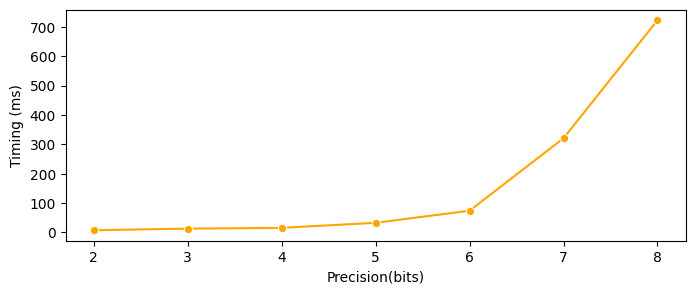
\includegraphics[width=0.8\linewidth]{img/to_harmonize/timings_pbs_precisions.png}
	\caption{TODO: remove the legend "CJP21". Maybe redraw it to have a taller figure}
	\label{fig:PBS_perfs}
\end{figure}



Intuitively, the reason is simple. When one wants to use a greater $p$, the torus must be sliced into more parts, that are thus smaller. When we switch the modulus to $2N$ in the bootstrapping, the ``windows'' of the accumulator polynomial gets smaller, so the bound on the noise to ensure correct bootstrapping must be smaller. To keep some room to enable the homomorphic capabilities of TFHE, one has to pick a greater value for the degree $N$. As this must be a power of two, it quickly reach values where the polynomial operations gets very slow.

Usually, PBS is not used for plaintext modulus greater than 8 bits. Some constructions exist in the literature to extend the capabilities of this algorithm to larger plaintext spaces, notably the WoP-PBS of \cite{AC:CLOT21}. In this thesis, we propose our own in Chapter \ref{chap:larger_lut}.




